\documentclass{article}

% packages
\usepackage[a4paper, margin=2cm]{geometry}
\usepackage{multicol}
\usepackage[utf8]{inputenc}
\usepackage[english]{babel}
\usepackage{minted}
\usepackage{pgfplots}

\newlength\figurewidth
\newlength\figureheight
\setlength\figurewidth{0.3\textwidth}
\setlength\figureheight{0.3\textwidth}

\begin{document}

    \begin{titlepage}
        \begin{center}
            \vspace*{2cm}
            
            {\huge \textbf{xCore-200 Cellular Automaton Farm}}
            
            \vspace{0.5cm}
            
            {\Large COMS20001 Concurrent Computing CW1}
            
            \vspace{0.5cm}
            
            {\large Team 6}
            
            \vspace{1cm}
            
            \hspace*{1cm} {\Large \textbf{Ruairi Fox}} \hfill {\Large \textbf{Liam Dalgarno}} \hspace*{1cm} \\~\\[-0.5em]
            \hspace*{1cm} MEng. Computer Science \hfill MEng. Computer Science  \hspace*{1cm} \\~\\[-1em]
            \hspace*{1cm} rf17160@bristol.ac.uk  \hfill ld17285@bristol.ac.uk  \hspace*{1cm} 
            
            \vspace{1cm}
            
            {\large \today}
        \end{center}
    \end{titlepage}

    \section{Functionality and Design}
    1 Page Max: Outline what functionality you have implemented, which problems you have solved with your implementation and how your program is designed to solve the problems efficiently and effectively
    \pagebreak

    \section{Tests and Experiments}
    (2 pages max): Show the result of the given 16x16 image after 2 rounds. Describe briefly the other experiments you carried out, provide a selection of appropriate results and output images. This must be done for at least the example images provided and for at least one example image of your own choosing (showcasing the merit of your system). List the important factors responsible for virtues and limitations of your system. 
    \pagebreak

    % ?? is a placeholder for a future citation :)
    \section{Critical Analysis}
    
    \begin{figure}
        \begin{center}
            % This file was created by matplotlib2tikz v0.6.18.
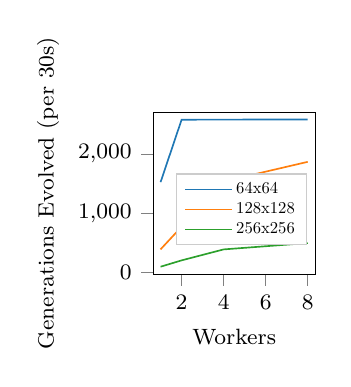
\begin{tikzpicture}

\definecolor{color0}{rgb}{0.12156862745098,0.466666666666667,0.705882352941177}
\definecolor{color1}{rgb}{1,0.498039215686275,0.0549019607843137}
\definecolor{color2}{rgb}{0.172549019607843,0.627450980392157,0.172549019607843}
\pgfplotsset{every tick label/.append style={font=\footnotesize}}
\begin{axis}[
height=\figureheight,
legend cell align={left},
legend entries={{64x64},{128x128},{256x256}},
legend style={nodes={scale=0.6, transform shape}, at={(0.95,0.4)}, anchor=east, draw=white!80.0!black},
tick align=outside,
tick pos=left,
width=\figurewidth,
x grid style={white!69.01960784313725!black},
xlabel={\footnotesize Workers},
xmin=0.65, xmax=8.35,
y grid style={white!69.01960784313725!black},
ylabel={\footnotesize Generations Evolved (per 30s)},
ymin=-30.2, ymax=2702.2
]
\addlegendimage{no markers, color0}
\addlegendimage{no markers, color1}
\addlegendimage{no markers, color2}
\addplot [semithick, color0]
table [row sep=\\]{%
1	1521 \\
2	2575 \\
4	2577 \\
8	2578 \\
};
\addplot [semithick, color1]
table [row sep=\\]{%
1	387 \\
2	769 \\
4	1533 \\
8	1864 \\
};
\addplot [semithick, color2]
table [row sep=\\]{%
1	94 \\
2	201 \\
4	386 \\
8	493 \\
};
\end{axis}

\end{tikzpicture}
            \hspace{1cm}
            % This file was created by matplotlib2tikz v0.6.18.
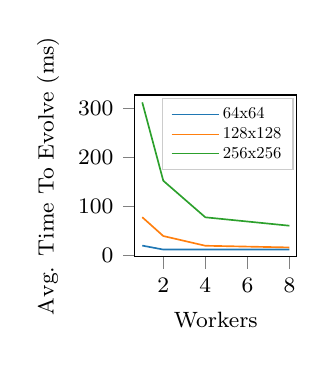
\begin{tikzpicture}

\definecolor{color0}{rgb}{0.12156862745098,0.466666666666667,0.705882352941177}
\definecolor{color1}{rgb}{1,0.498039215686275,0.0549019607843137}
\definecolor{color2}{rgb}{0.172549019607843,0.627450980392157,0.172549019607843}
\pgfplotsset{every tick label/.append style={font=\footnotesize}}
\begin{axis}[
height=\figureheight,
legend cell align={left},
legend entries={{64x64},{128x128},{256x256}},
legend style={nodes={scale=0.6, transform shape}, draw=white!80.0!black},
tick align=outside,
tick pos=left,
width=\figurewidth,
x grid style={white!69.01960784313725!black},
xlabel={\footnotesize Workers},
xmin=0.65, xmax=8.35,
y grid style={white!69.01960784313725!black},
ylabel={\footnotesize Avg. Time To Evolve (ms)},
ymin=-3.424, ymax=327.544
]
\addlegendimage{no markers, color0}
\addlegendimage{no markers, color1}
\addlegendimage{no markers, color2}
\addplot [semithick, color0]
table [row sep=\\]{%
1	19.69 \\
2	11.63 \\
4	11.64 \\
8	11.62 \\
};
\addplot [semithick, color1]
table [row sep=\\]{%
1	77.72 \\
2	39.27 \\
4	19.4 \\
8	15.91 \\
};
\addplot [semithick, color2]
table [row sep=\\]{%
1	312.5 \\
2	152.28 \\
4	77.52 \\
8	60.36 \\
};
\end{axis}

\end{tikzpicture}
        \end{center}
        \vspace{-2mm}
        \caption{Effect of increasing worker count on processing speed.}
        \label{fig:workers}
    \end{figure}

    Our system can process a \verb|1024x1024| image across 8 workers, and can evolve a single generation of a \verb|256x256| board in 60ms ??. The xCore-200 is harshly limited by its I/O speed (reading of a \verb|1024x1024| file can take many minutes); we chose to use \verb|64x64| to \verb|256x256| in the sample data as it is much faster to read from disk while also able to show trends. Figure \ref{fig:workers} shows that increasing the number of workers also increases the effective processing speed. This relationship is \textit{somewhat} linear: doubling the workers from 1, 2, to 4 on the \verb|128x128| and \verb|256x256| images seem to also halve the average generation time. However, the relationship is weaker for \verb|64x64| and 8 workers across all image sizes, which implies that the system is bottlenecked by some other factor. We believe that it is bottlenecked by both processing speed and channel communication with the distributor, since it needs to collect the `ghost rows' before the generation can advance. \\

    \begin{figure}[h]
        \begin{center}
            \begin{tabular}{|c|c|c|}
                \hline Workers & Size & Avg. Generation Time (ms) \\
                \hline 1 & 64x64 & 19.69 \\
                2 & 64x64 & 11.63 \\
                4 & 64x64 & 11.64 \\
                8 & 64x64 & 11.62 \\
                1 & 128x128	& 77.72 \\
                2 & 128x128	& 39.27 \\
                4 & 128x128 & 19.40 \\
                8 & 128x128 & 15.91 \\
                1 & 256x256	& 312.50 \\
                2 & 256x256	& 152.28 \\
                4 & 256x256	& 77.52 \\
                8 & 256x256	& 60.36 \\
                \hline
            \end{tabular}
        \end{center}
    \end{figure}

    Hard channels are channels between cores while soft channels are between threads on the same core, so a way to reduce the effect of the bottleneck would be to prefer \textbf{soft channel} communcation over \textbf{hard channel} communication. Soft channels have lower latency ??
\end{document}